\documentclass[a4paper,12pt]{report}
\usepackage[T2A]{fontenc}
\usepackage[utf8x]{inputenc}
\usepackage[english,russian]{babel}%используем русский и английский языки с переносами
\usepackage{mathptmx}
%\usepackage{times} 
\usepackage{amssymb,amsfonts,amsmath,amsthm,mathtext,cite,enumerate,float} %подключаем нужные пакеты расширений

\ifx\pdfoutput\undefined
\usepackage{graphicx}
\else
\usepackage[pdftex]{graphicx}
\fi
\graphicspath{{images/}}%путь к рисункам

%\usepackage{indentfirst} % отделять первую строку раздела абзацным отступом тоже
\usepackage[usenames,dvipsnames]{color} % названия цветов
\usepackage{makecell}
\usepackage{multirow} % улучшенное форматирование таблиц
\usepackage{ulem} % подчеркивания
 
\linespread{1.3} % полуторный интервал
%\renewcommand{\rmdefault}{ftm} % Times New Roman
\frenchspacing

\makeatletter
\renewcommand{\@biblabel}[1]{#1.} % Заменяем библиографию с квадратных скобок на точку:
\makeatother

\usepackage{geometry} % Меняем поля страницы
\geometry{left=3cm}% левое поле
\geometry{right=1cm}% правое поле
\geometry{top=1cm}% верхнее поле
\geometry{bottom=1.7cm}% нижнее поле


\usepackage{titlesec}
\titleformat{\chapter}[block]
{\normalfont\bfseries}{\thechapter}{1em}{\Large}
\titleformat{\section}[block]
{\normalfont\bfseries}{\thesection}{.5em}{\Large}

\renewcommand{\theenumi}{\arabic{enumi}}% Меняем везде перечисления на цифра.цифра
\renewcommand{\labelenumi}{\arabic{enumi}}% Меняем везде перечисления на цифра.цифра
\renewcommand{\theenumii}{.\arabic{enumii}}% Меняем везде перечисления на цифра.цифра
\renewcommand{\labelenumii}{\arabic{enumi}.\arabic{enumii}.}% Меняем везде перечисления на цифра.цифра
\renewcommand{\theenumiii}{.\arabic{enumiii}}% Меняем везде перечисления на цифра.цифра
\renewcommand{\labelenumiii}{\arabic{enumi}.\arabic{enumii}.\arabic{enumiii}.}% Меняем везде перечисления на цифра.цифра

\setcounter{tocdepth}{2}

\usepackage{color}
\definecolor{white}{rgb}{1,1,1}
\definecolor{gray}{rgb}{0.5,0.5,0.5}

\usepackage{listings}
\lstset{
language=R,
basicstyle=\scriptsize\ttfamily,
commentstyle=\ttfamily\color{gray},
numbers=left,
numberstyle=\ttfamily\color{gray}\footnotesize,
stepnumber=1,
numbersep=10pt,
backgroundcolor=\color{white},
showspaces=false,
showstringspaces=false,
showtabs=false,
frame=single,
tabsize=2,
captionpos=b,
breaklines=true,
breakatwhitespace=false,
title=\lstname,
escapeinside={},
keywordstyle={},
morekeywords={}
}

\overfullrule=2cm

\begin{document}
\begin{titlepage}
\begin{center}
РОССИЙСКАЯ ФЕДЕРАЦИЯ\\
Московская область \\ \vspace{1cm}
Филиал «Котельники»\\
Государственного бюджетного образовательного учреждения\\
высшего образования Московской области\\
«Международный университет природы, общества и человека «Дубна»\\
Кафедра «Информационных технологий в управлении»

\vspace{2.5em}

Курсовая работа\\
по дисциплине «Теория вероятностей и математическая статистика»\\
Вариант 15


\end{center}

\vspace{6em}
 
\begin{flushright}
Выполнил:\\
Студент гр. ИВТ-21\\ 
Юнькин Петр Дмитриевич\\
Преподаватель:\\
Артамонов Юрий Николаевич

\end{flushright}

 
\vspace{\fill}

\begin{center}
Котельники 2015
\end{center}
\end{titlepage}
\tableofcontents
\chapter{\textbf{Введение}}
Теория вероятности - математическая наука, позволяющая по вероятностям одних случайных событий находить вероятности других случайных событий, связанных каким-либо образом с первыми. Утверждение о том, что какое-либо событие наступает с вероятностью, равной, например, ½, ещё не представляет само по себе окончательной ценности, так как мы стремимся к достоверному знанию. Окончательную познавательную ценность имеют те результаты теории вероятностей, которые позволяют утверждать, что вероятность наступления какого-либо события А весьма близка к единице или (что то же самое) вероятность не наступления события А весьма мала. В соответствии с принципом "пренебрежения достаточно малыми вероятностями"  такое событие справедливо считают практически достоверным. Поэтому можно также сказать, что теория вероятностей есть математическая наука, выясняющая закономерности, которые возникают при взаимодействии большого числа случайных факторов.\\
Возможность применения методов теории вероятностей к изучению статистических закономерностей, относящихся к весьма далёким друг от друга областям науки, основана на том, что вероятности событий всегда удовлетворяют некоторым простым соотношениям, о которых будет сказано ниже. Изучение свойств вероятностей событий на основе этих простых соотношений и составляет предмет теории вероятностей. Наиболее просто определяются основные понятия теории вероятностей как математической дисциплины в рамках так называемой элементарной теории вероятностей.\\
\chapter{\textbf{Цель курсовой работы}}
Целью данной курсовой работы является углубление теоретических знаний по курсу «Теория вероятностей и математическая статистика», получение навыков самостоятельного решения прикладных задач как на основе теоретических знаний, так и экспериментально с помощью среды R.\\
Курсовая работа содержит решение задач по основным теоремам теории вероятностей и  решение задач по разделу законы распределения случайных величин, оценка их числовых характеристик.

\chapter{Основная часть}
\section{Часть 1}
\subsection{Условия задач}
Задача 16\\

Сейфовый замок имеет 4 диска с пятью секторами, на
каждом из которых записана одна из цифр от 0 до 4 . Какова
вероятность открыть замок сейфа, набрав 4 цифры наугад?\\


Задача 46\\

Вероятность попадания в кольцо первого игрока – 0,7, а
второго игрока – 0,8. Игроки бросают мяч по два раза независимо друг от друга. Какова вероятность того, что мяч попадет в
кольцо два раза?\\


Задача 58\\

Имеются две коробки с мячами для тенниса. В первой коробке 7 красных и 8 зелёных мячей; во второй – 9 красных и 11
зелёных. Из первой и второй коробок, не глядя, берут по одному
мячу и кладут в третью коробку. Мячи в третьей коробке перемешивают и берут наугад один мяч. Определить вероятность
того, что этот мяч зелёный.\\


Задача 75\\

Для посева заготовлены семена 4 видов клёна. Причем,
22 % всех семян клёна 1-го вида; 33 % – 2-го вида; 32 % – 3-
го вида; 13 % – 4-го вида. Вероятность всхожести для семян
первого вида равна 0,69; для второго – 0,74; для третьего – 0,43;
для четвёртого – 0,38. Найти вероятность того, что наугад взятое
семечко взойдёт.\\


Задача 78\\

В группе спортсменов 12 метателей снарядов, 17 бегунов и
19 прыгунов. Вероятность выполнить квалификационную норму
для метателя снаряда равна 0,71; для бегуна – 0,89; для прыгуна – 0,73. Найти вероятность того, что спортсмен, выбранный
наугад, выполнит норму.\\


Задача 88\\

В лесхозе 50 \% посадок составляет сосна; 40 \% береза и 10 43
\% ель. Вероятность поражения грибковыми заболеваниями для
этих деревьев составляет 0,3; 0,6 и 0,8 соответственно. При санитарном осмотре было выбраковано дерево. Какова вероятность
того, что это дерево ель?\\

\subsection{Теоретическое решение}
Задача 16.\\
Задача решается с помощью классического определения вероятности.\\
Формула классической вероятности имеет следующий вид:\\
\begin{center}
$P=\frac{m}{n}$,\\
\end{center}
где $m$-число случаев, благоприятных для данного
события, а $n$-полная группа равновозможных и несовместных случаев.\\
В сейфовом замке диски независимы друг от друга. Каждый диск имеет по 5 секторов. Следовательно имеем $m=1$ и $n=5$ для каждого из дисков.\\
Пусть $A$ - событие открытия сейфа. Тогда для нахождения $P(A)$ требуется одновременное наступление событий, соответствующих угадыванию цифры на каждом диске:\\
\begin{center}
$P(A)=\frac{1}{5}\cdot\frac{1}{5}\cdot\frac{1}{5}\cdot\frac{1}{5}=\frac{1}{625}=0.0016$\\
\end{center}
Задача 46.\\
В данной задаче применяются теоремы сложения и умножения вероятностей.\\
Пусть $A$ и $B$ - события попадания в кольцо соответственно первого и второго игроков. Тогда вероятности их попадания:
\begin{center}
$P(A)=0.7$\\
$P(B)=0.8$\\
\end{center}
Для подсчета вероятности попадания мяча в кольцо 2 раза из 4 нужно сложить вероятности каждого такого случая.\\
Перечислим данные случаи:
\begin{enumerate}
\item Случай когда первый игрок попал 2 раза, а второй - ни разу. \\$P(A)\cdot P(A)\cdot P(\overline{B})\cdot P(\overline{B})$\\
\item Случай когда второй игрок попал 2 раза, а первый - ни разу. \\$ P(\overline{A})\cdot P(\overline{A})\cdot P(A)\cdot P(A)$\\
\item Случаи когда и первый и второй игроки попали по одному разу(Всего 4 таких случая из-за возможности разных комбинаций.\\
$ P(\overline{A})\cdot P(A)\cdot P(B)\cdot P(\overline{B})$\\
$ P(A)\cdot P(\overline{A})\cdot P(B)\cdot P(\overline{B})$\\
$ P(\overline{A})\cdot P(A)\cdot P(\overline{B})\cdot P(B)$\\
$ P(A)\cdot P(\overline{A})\cdot P(\overline{B})\cdot P(B)$\\
\end{enumerate}
Проведем окончательные численные расчеты:\\
$P=0.7\cdot 0.7\cdot 0.2\cdot 0.2+0.3\cdot 0.3\cdot 0.8\cdot 0.8+4\cdot(0.7\cdot 0.3\cdot 0.8\cdot 0.2)=0.0196+0.0576+0.1344=0.2256$\\

Задача 59.\\
Темой задачи ялвяется полная вероятность.\\
Формула полной вероятности выглядит так:\\
$$P(A)=\sum_{i=0}^{n} P(H_i)P(A/H_i)$$\\
Перекладывание из первой коробки зеленого мяча (событие $H_1$ - первая гипотеза), красного мяча (событие $H_2$ - вторая гипотеза) и соответственно зеленого (событие $H_3$ - третья гипотеза) и красного (событие $H_4$ - четвертая гипотеза) из второй коробки составляют две полные группы независимых событий.\\
Их вероятности равны:\\
\begin{center}
$P(H_1)=\frac{8}{15}$\\
$P(H_2)=\frac{7}{15}$\\
$P(H_3)=\frac{11}{20}$\\
$P(H_4)=\frac{9}{20}$\\
\end{center}
Чтобы посчитать вероятность вытаскивания из третьей коробки зеленого мяча, рассмотрим 3 случая:\\
\begin{enumerate}
\item Из первой коробки достали зеленый мяч, а из второй - красный.
\item Из первой коробки достали красный мяч, а из второй - зеленыый.
\item Из обеих коробок достали по зеленому мячу.
\end{enumerate}
Пусть $A$- событие вытаскивания из третьей коробки зеленого мяча.\\
Найдем условные вероятности для каждого из вышестоящих случаев:\\
В первом и втором случаях в третьей корзине окажутся один зеленый и один красный мячи:\\
\begin{center}
$P(A/H_1 H_4)=P(A/H_2 H_3)=\frac{1}{2}$\\
\end{center}
В третьем случае в коробке будут находиться только зеленые мячи:\\
\begin{center}
$P(A/H_1 H_3)=1$\\
\end{center}
Выполним оставшиеся расчеты по формуле полной вероятности:\\
\begin{center}
$P(A)=\frac{8}{15}\cdot \frac{9}{20}\cdot \frac{1}{2} + \frac{7}{15}\cdot \frac{11}{20}\cdot \frac{1}{2} + \frac{8}{15}\cdot \frac{11}{20}=0.12 + 0.128(3) + 0.29(3)= 0.541 $\\
\end{center}
Задача 75\\
Задача решается методом, аналогичным предыдущей задачи.\\
Пусть $A$ - событие всхода семечка.\\
Пусть $H_1$,$H_2$,$H_3$,$H_4$ - гипотезы, соответствующие выпадению семечка клена каждого из 4 видов.\\
Распишем вероятности  гипотез каждого вида:\\

\begin{center}
$P(H_1)=0.22$ \\
$P(H_2)=0.33$ \\
$P(H_3)=0.32$ \\
$P(H_4)=0.13$ \\
\end{center}
Также запишем условные вероятности всхода каждого вида семян:\\
\begin{center}
$P(A/H_1)=0.69$\\
$P(A/H_2)=0.74$\\
$P(A/H_3)=0.43$\\
$P(A/H_4)=0.38$\\
\end{center}
Для нахождения вероятности того, что семечко, взятое наугад, взойдет воспользуемся формулой полной вероятности:\\
$P=0.22\cdot 0.69 + 0.33\cdot 0.74 + 0.32 \cdot 0.33 + 0.13\cdot 0.38=0.583$\\

Задача 78\\
Задача решается аналогично двум вышестоящим.\\
Пусть $A$ - событие выполнения нормы спортсменом.\\
Пусть $H_1$,$H_2$,$H_3$ - гипотезы, соответствующие выпадению каждого типа спортсменов.\\
Вероятности гипотез каждого вида:\\
\begin{center}
$P(H_1)=\frac{12}{48}=\frac{1}{4}$ \\
$P(H_2)=\frac{17}{48}$ \\
$P(H_3)=\frac{19}{48}$ \\
\end{center}
Условные вероятности выполнения нормы спортсменами:\\
\begin{center}
$P(A/H_1)=0.71$\\
$P(A/H_2)=0.89$\\
$P(A/H_3)=0.73$\\
\end{center}

Для нахождения вероятности того, что спортсмен, взятый наугад, выполнит норму воспользуемся формулой полной вероятности:\\
$P=\frac{1}{4}\cdot 0.71 + \frac{17}{48}\cdot 0.89 + \frac{19}{48}\cdot 0.73=0.7816$\\
\\Задача 88.\\
В задаче используется формула Байеса (теорема гипотез).\\
Пусть имеется полная группа несовместных гипотез $H_1,H_2,\cdots,H_n$, известны вероятности $P(H_i)$,  $i=\overline{1,n}$ этих гипотез до опыта и условные вероятности
$P(A/H_i)$  события $A$, которое может произойти лишь совместно с одной гипотезой.
Произведён опыт, в результате которого событие $A$ произошло, тогда условные вероятности $P(H_i/A)$ вычисляются по формуле:\\
\begin{center}
$P(H_i/A)=\frac{P(H_i)P(A/H_i)}{P(A)}$,
где $$P(A)=\sum_{i=0}^{n} P(H_i)P(A/H_i)$$\\
\end{center}
Пусть $A$ - событие выбраковки дерева.\\
Пусть гипотезы $H_1$,$H_2$,$H_3$ соответствуют выпадению каждого вида дерева.\\
Имеем следующие вероятности данных гипотез:\\
\begin{center}
$P(H_1)=0.5$\\
$P(H_2)=0.4$\\
$P(H_3)=0.1$\\
\end{center}
Условные вероятности выбраковки каждого вида дерева:\\
\begin{center}
$P(A/H_1)=0.3$\\
$P(A/H_2)=0.6$\\
$P(A/H_3)=0.8$\\
\end{center}
Вычисляем $P(A)$ и подставляем в формулу Баейса:\\
\begin{center}
$P(A)=0.5\cdot 0.3+0.4\cdot 0.6+0.1\cdot 0.8=0.47$\\
$P(H_3/A)=\frac{P(H_3)P(A/H_3)}{P(A)}=\frac{0.1\cdot 0.8}{0.47}=0.1702$\\
\end{center}
\newpage


\subsection{Программное решение}
Задача 16
\begin{lstlisting}[language=R,basicstyle=\normalsize]
N<-100000
m<-0
for(i in 1:N)
{
n<-0;
for(j in 1:4)
	{
	x<-sample(1:5,1);
	if(x==1)n<-n+1;
	}
if(n==4)m<-m+1;
}
m/N
\end{lstlisting}
Задача 46
\begin{lstlisting}[language=R,basicstyle=\normalsize]
N<-100000
a<-0
for(i in 1:N)
{
    n<-0
    m<-0
    x<-runif(2,0,100)
    y<-runif(2,0,100)
    for(j in 1:2)
    {
        if(x[j]<70)n<-n+1;
        if(y[j]<80)m<-m+1;
    }
    if(n==2 && m==0)a<-a+1;
    if(n==1 && m==1)a<-a+1;
    if(n==0 && m==2)a<-a+1;
}
a/N
\end{lstlisting}
\newpage
Задача 59
\begin{lstlisting}[language=R,basicstyle=\normalsize]
N<-1000000
a<-0
for(i in 1:N)
{
x<-sample(1:15,1)
y<-sample(1:20,1)
z<-sample(1:2,1)
if(x<8 && y>9 && z==1)a<-a+1;
if(x>7 && y<10 && z==1)a<-a+1;
if(x>7 && y>9)a<-a+1;
}
a/N
\end{lstlisting}
Задача 75
\begin{lstlisting}[language=R,basicstyle=\normalsize]
N<-1000000
a<-0
for(i in 1:N)
{
x<-sample(1:100,1);
s1<-runif(1,0,1);
s2<-runif(1,0,1);
s3<-runif(1,0,1);
s4<-runif(1,0,1);
if(x<23 && s1<=0.69)a<-a+1;
if(x>22 && x<56 && s2<=0.74)a<-a+1;
if(x>55 && x<88 && s3<=0.43)a<-a+1;
if(x>87 && s4<=0.38)a<-a+1;
}
a/N
\end{lstlisting}
\newpage
Задача 78
\begin{lstlisting}[language=R,basicstyle=\normalsize]
N<-1000000
a<-0
for(i in 1:N)
{
x<-sample(1:48,1)
s1<-runif(1,0,1);
s2<-runif(1,0,1);
s3<-runif(1,0,1);
if(x<13 && s1<=0.71)a<-a+1;
if(x>12 && x<30 && s2<=0.89)a<-a+1;
if(x>29 && s3<=0.73)a<-a+1;
}
a/N
\end{lstlisting}
Задача 88
\begin{lstlisting}[language=R,basicstyle=\normalsize]
N<-1000000
a<-0
b<-0
for(i in 1:N)
{
x<-sample(1:10,1)
s1<-runif(1,0,1);
s2<-runif(1,0,1);
s3<-runif(1,0,1);
if(x<6 && s1<=0.3)a<-a+1;
if(x>5 && x<10 && s2<=0.6)a<-a+1;
if(x>9 && s3<=0.8){a<-a+1;b<-b+1;}
}
b/a
\end{lstlisting}
\newpage
\section{Часть 2}
\subsection{Условия задач}
Задание 1\\

Даны реализации случайной величины с известным законом распределения. Построить гистограмму относительных частот по выборке. Получить оценки характеристик распределения, на основании полученных характеристик оценить вероятность попадания случайной величины в заданный интервал (a; b).\\


Распределение: нормальное;\\
Интервал: a = 9, b = 16;\\
Реализации: 7.323809; 6.619512; 6.751731; 6.038427; 9.065843;\\
7.419849; 4.316773; 7.840065; 6.305318; 10.070025; 4.362429; 4.820292;\\
1.033636; 4.095188; 2.540600; 9.260781; 12.624193; 6.541842; 2.956328;\\
5.398058; 1.062041; 8.063377; 10.035916; 4.562224; 9.073952; 4.447496;\\
9.399037; 5.142934; 6.786499; 5.963823.\\


Задание 2\\

В соответствии с вариантом найти и построить функцию
распределения дискретной случайной величины Z, полученной
из независимых случайных величин X, Y , найти математическое
ожидание, дисперсию, стандартное отклонение и моду дискретной случайной величины Z (при построении графика использовать средства R, при нахождении математического ожидания и
дисперсии, кроме теоретического решения, предложить численное решение в среде R).\\

 \begin{center}
 $Z = X\cdot sin(Y)$\\
 \end{center}


\begin{table}[!h]
\centering
%\caption{My caption}
\label{my-label}
\begin{tabular}{|c|c|c|c|c|c|}
\hline
X     & 5          & 6          & 10         & 16         & 17         \\ \hline
$P_x$ & 0.1553912  & 0.2683355  & 0.1841288  & 0.2818739  & 0.1102706  \\ \hline
Y     & 5          & 6          & 10         & 16         & 17         \\ \hline
$P_y$ & 0.31514155 & 0.08008699 & 0.28486710 & 0.12811419 & 0.19179018 \\ \hline
\end{tabular}
\end{table}
\newpage
\subsection{Программное решение}
Задание 1\\
Нормальное распределение\\
Нормальным называется распределение вероятностей непрерывной
случайной величины, плотность распределения которой
\begin{center}
$$f(x)=\frac{1}{\sigma\sqrt{2\pi}}e^{-\frac{(x-m)^2}{2\sigma^2}} (-\infty<x<\infty)$$,\\
\end{center}
где $m$,$\sigma$– параметры нормального распределения, при этом $\sigma>0$.\\
Параметр $m$ представляет собой математическое ожидание нормального распределения.\\
Параметр $\sigma$ – среднее квадратическое отклонение нормального распределения.\\
Дисперсия нормального закона равна
\begin{center}
$D(X)=\sigma^2$\\
\end{center}
Функция нормального распределения
\begin{center}
$$F(x)=\frac{1}{\sigma\sqrt{2\pi}}\int_{-\infty}^{x}e^{-\frac{(x-m)^2}{2\sigma^2}}dx$$\\
\end{center}
Вероятность попадания нормально распределенной случайной величины на интервал $(a,b)$ равна
\begin{center}
$$P(a < X < b) = F(b) − F(a)$$
\end{center}
\newpage
\begin{lstlisting}[language=R,basicstyle=\normalsize]
x<-c(7.323809, 6.619512, 6.751731, 6.038427, 9.065843,
     7.419849, 4.316773, 7.840065, 6.305318, 10.070025, 4.362429, 4.820292,
     1.033636, 4.095188, 2.540600, 9.260781, 12.624193, 6.541842, 2.956328,
     5.398058, 1.062041, 8.063377, 10.035916, 4.562224, 9.073952, 4.447496,
     9.399037, 5.142934, 6.786499, 5.963823)

mean(x)
[1] 6.330733
sd(x)
[1] 2.718041
var(x)
[1] 7.387745
pnorm(16,mean(x),sd(x))-pnorm(9,mean(x),sd(x))
[1] 0.162849
hist(x)
\end{lstlisting}
%\newpage
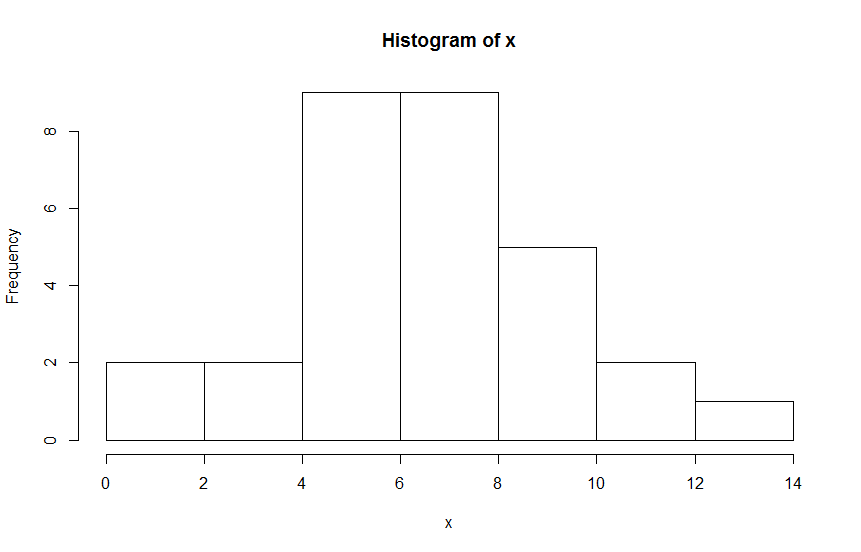
\includegraphics[scale=0.5]{Hist1.png}\\
\newpage
Задание 2\\
\begin{center}
 $Z = X\cdot sin(Y)$\\
 \end{center}
Составим ряд распределения случайной величины $Z$. Для этого для каждого $X$ подставим в формулу каждое значение $Y$, затем для полученных значений посчитаем вероятности, умножив соответствующую вероятность $X$ на вероятность $Y$. Получаем следующие таблицы.\\
\begin{lstlisting}[language=R,basicstyle=\normalsize]
x<-c(5,6,10,16,17)
y<-x
a<-matrix(0,5,5)
for(i in 1:length(x))
    for(j in 1:length(y))
        a[i,j]<-x[i]*sin(y[j])
print(a)
           [,1]      [,2]      [,3]      [,4]       [,5]
[1,]  -4.794621 -1.397077 -2.720106 -1.439517  -4.806987
[2,]  -5.753546 -1.676493 -3.264127 -1.727420  -5.768385
[3,]  -9.589243 -2.794155 -5.440211 -2.879033  -9.613975
[4,] -15.342788 -4.470648 -8.704338 -4.606453 -15.382360
[5,] -16.301713 -4.750063 -9.248359 -4.894356 -16.343757

px<-c(0.1553912,0.2683355,0.1841288,0.2818739,0.1102706)
py<-c(0.31514155,0.08008699,0.28486710,0.12811419,0.19179018)
b<-matrix(0,5,5)
for(i in 1:length(px))
    for(j in 1:length(py))
        b[i,j]<-px[i]*py[j]
print(b)
           [,1]       [,2]       [,3]       [,4]       [,5]
[1,] 0.04897022 0.01244481 0.04426584 0.01990782 0.02980251
[2,] 0.08456367 0.02149018 0.07643996 0.03437759 0.05146411
[3,] 0.05802664 0.01474632 0.05245224 0.02358951 0.03531410
[4,] 0.08883018 0.02257443 0.08029660 0.03611205 0.05406065
[5,] 0.03475085 0.00883124 0.03141247 0.01412723 0.02114882
\end{lstlisting}
Найдем математическое ожидание, дисперсию, стандартное отклонение и моду дискретной случайной величины Z:\\
$$M(Z)=\sum_{i=0}^{n}x_i p_i$$
$$D(Z)=M(Z^2)-(M(Z))^2$$
$$\sigma=\sqrt{D(Z)}$$\\
Модой случайной величины называется ее наиболее вероятное  значение. Для дискретной случайной величины - это значение, встречающееся с наибольшей частотой.По ряду распределения можно выявить, что модой случайной величины $Z$ является значение -15.342788.\\
\begin{lstlisting}[language=R,basicstyle=\normalsize]
Z<-c(-4.794621, -1.397077, -2.720106, -1.439517,  -4.806987,
     -5.753546, -1.676493, -3.264127, -1.727420,  -5.768385,
     -9.589243, -2.794155, -5.440211, -2.879033,  -9.613975,
     -15.342788, -4.470648, -8.704338, -4.606453, -15.382360,
     -16.301713, -4.750063, -9.248359, -4.894356, -16.343757)
P<-c(0.04897022, 0.01244481, 0.04426584, 0.01990782, 0.02980251,
     0.08456367, 0.02149018, 0.07643996, 0.03437759, 0.05146411,
     0.05802664, 0.01474632, 0.05245224, 0.02358951, 0.03531410,
     0.08883018, 0.02257443, 0.08029660, 0.03611205, 0.05406065,
     0.03475085, 0.00883124, 0.03141247, 0.01412723, 0.02114882)

m<-0
for(i in 1:length(Z))
    m<-Z[i]*P[i]+m
print(m)#M(Z)
[1] -7.437683
m2<-0
for(i in 1:length(Z))
    m2<-Z[i]*Z[i]*P[i]+m2
print(m2)#M(Z^2)
[1] 77.27161
d<-m2-m*m
print(d)#D(Z)
[1] 21.95249
sigma<-sqrt(d)
print(sigma)
[1] 4.685349
\end{lstlisting}
Запишем значения функции распределения в таблицу и построим ее график.\\ 
\begin{table}[!h]
\centering
%\caption{My caption}
\label{my-label}
\begin{tabular}{|l|l|l|}
\hline
\multicolumn{1}{|c|}{X\textless=0}         & F= & 0          \\ \hline
-16.343757\textless X\textless=-16.301713  & F= & 0.02114882 \\ \hline
-16.301713\textless X\textless=-15.382360  & F= & 0.05589967 \\ \hline
-15.382360\textless X\textless=-15.342788  & F= & 0.10996032 \\ \hline
-15.342788\textless X\textless=-9.613975   & F= & 0.1987905  \\ \hline
-9.613975\textless X\textless=-9.589243    & F= & 0.23411046 \\ \hline
-9.589243\textless X\textless=-9.248359    & F= & 0.29213134 \\ \hline
-9.248359\textless X\textless=-8.704338    & F= & 0.32354371 \\ \hline
-8.704338\textless X\textless=-5.768385    & F= & 0.40384031 \\ \hline
-5.768385\textless X\textless=-5.753546    & F= & 0.45530442 \\ \hline
-5.753546\textless X\textless=-5.440211    & F= & 0,53986809 \\ \hline
-5.440211\textless X\textless=-4.894356    & F= & 0.59232033 \\ \hline
-4.894356\textless X\textless=-4.806987    & F= & 0.60644756 \\ \hline
-4.806987\textless X\textless=-4.794621    & F= & 0.63625007 \\ \hline
-4.794621\textless X\textless=-4.750063    & F= & 0.68522029 \\ \hline
-4.750063\textless X\textless=-4.606453    & F= & 0.69405153 \\ \hline
-4.606453\textless X\textless=-4.470648    & F= & 0.73016358 \\ \hline
-4.470648\textless X\textless=-3.264127    & F= & 0.75273801 \\ \hline
-3.264127\textless X\textless=-2.879033    & F= & 0.82917797 \\ \hline
-2.879033\textless X\textless=-2.794155    & F= & 0.85276748 \\ \hline
-2.794155\textless X\textless=-2.720106    & F= & 0.8675138  \\ \hline
-2.720106\textless X\textless=-1.727420    & F= & 0.91177964 \\ \hline
-1.727420\textless X\textless=-1.676493    & F= & 0.94615723 \\ \hline
-1.676493\textless X\textless=-1.439517    & F= & 0.96764741 \\ \hline
-1.439517\textless X\textless=-1.397077    & F= & 0.98755523 \\ \hline
\multicolumn{1}{|c|}{-1.397077 < X} & F= & 1          \\ \hline
\end{tabular}
\end{table}
\newpage
\begin{figure}[!h]
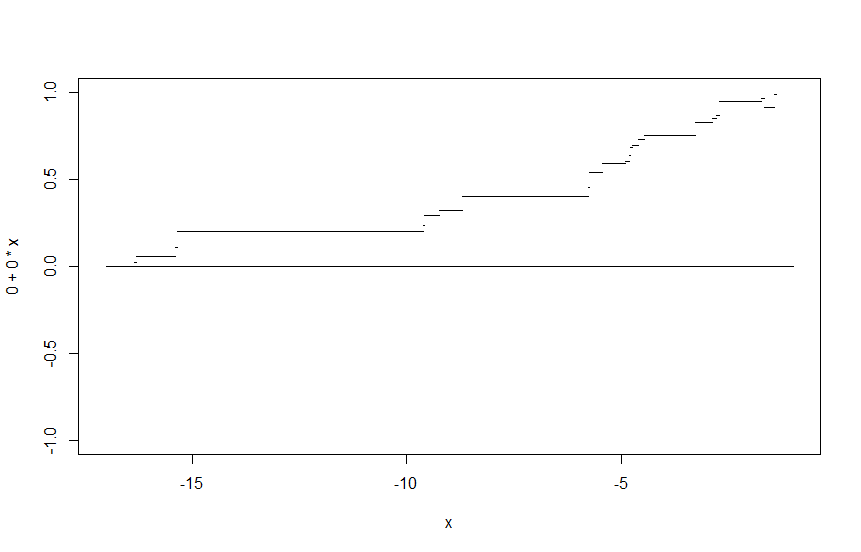
\includegraphics[scale=0.75,angle=90]{Rplot.png}\\
\end{figure}

\chapter{Выводы}
В ходе выполнения лабораторной работы были укреплены знания по курсу «Теория вероятностей и математическая статистика». Также во время решения задач были получены навыки по программированию на языке R для последующего решения повседневных задач. Работа выполнена полностью.\\
Работа была оформлена с помощью системы компьютерной верстки \TeX, повсеместно используещейся для оформления различных работ и публикаций.\\
Теория вероятности и ее основы используются во многих других математических, информационных и других дисциплинах.\\
На текущий момент необходимость изучения теории вероятности для современного технического специалиста неоспорима.

\chapter{Список литературы}
\begin{enumerate}
\item Гмурман В.Е. Руководство к решению задач по теории вероятностей и математической статистике: учеб.пособие -
М.: ИД Юрайт, 2010. - 404 с.\\
\item  Данилин Г. А. и др. Элементы теории вероятностей с Excel:
Практикум для студентов всех специальностей МГУЛа.,/
Г. А. Данилин, В. М. Курзина, П. А. Курзин, О. М. Полещук. М.: МГУЛ, 2004. 87 с.: ил.\\
\item  Вентцель Е. С. Задачи и упражнения по теории вероятностей: Учеб. пособие для студ. втузов / Е. С. Вентцель, Л.\\
А. Овчаров. — 5-е изд., испр. — М.: Издательский центр
«Академия», 2003. — 448 с.\\
\item  Венцель Е.С. Теория вероятностей: учебник - М.: Физ-мат
лит., 1958. - 464 с.\\
\item Гнеденко Б. В. и Хинчин А. Я., Элементарное введение в теорию вероятностей, 3 изд.,К. - Л.,2008.\\
\item Луговая И. Н., Курс теории вероятностей, 4 изд., М., 2001.\\
\item Феллер В., Введение в теорию вероятностей и её приложение (Дискретные распределения), пер. с англ., 2 изд., т. 1-2,К.,2003.\\
\item Бернштейн С. Н., Теория вероятностей, 4 изд.,К. - Л., 2003.\\
\item А.А.Савельев и др., Основные понятия языка R Учебно-методическое пособие, Казань 2007
\end{enumerate}
\end{document}
